\section{Вычислительные эксперименты}
    \subsection{Алгоритм}
        Для расчётов и визуализации был использован язык Python с библиотеками numpy и matplotlib, в котором был реализован метод Рунге-Кутта.

        \lstinputlisting[language=Python,
        captionpos=t,
        style=colored,
        basicstyle=\footnotesize\dejavu,
        frame=lines]{src/2.py}

    \subsection{Модель без терморегулятора}
        \begin{figure}[H]
            \centering
            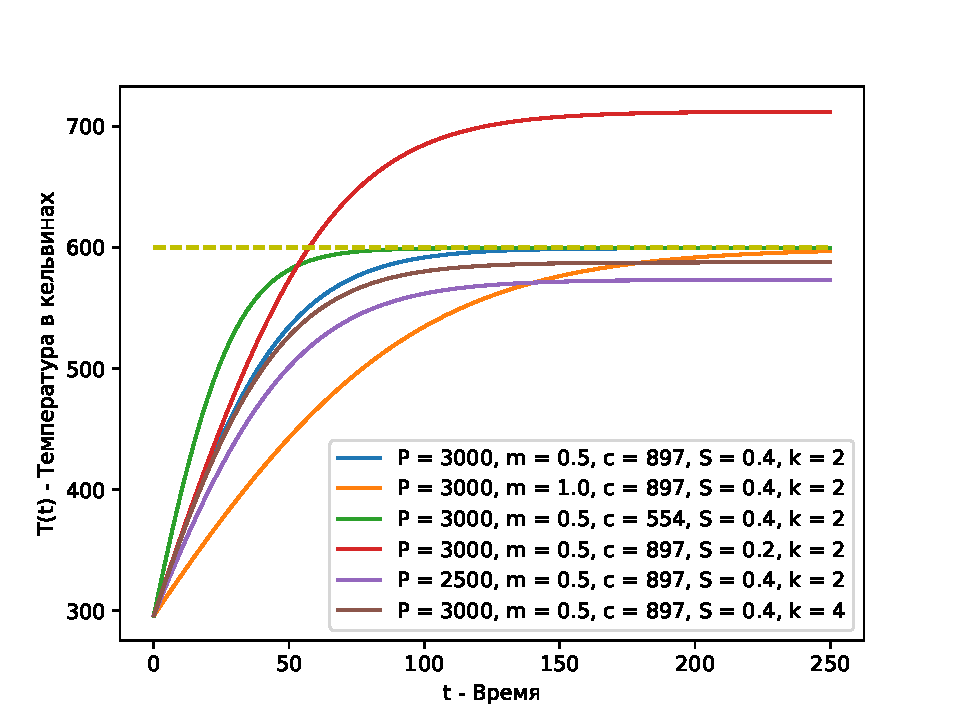
\includegraphics[width=17cm]{pictures/utug1.pdf}
            \caption{Графики моделей при $T_0 = 296$.}
        \end{figure}

        На графике (Рис. 1) построены несколько моделей с указанными параметрами, а также жёлтый пунктир на отметке $T = 600$ -- округлённое значение, найденное при анализе.
        
        Как можно увидеть, первые три модели, которые отличаются только массой и удельной теплоёмкостью, возрастают до определённого значения -- точки равновесия. 
        
        Остальные модели различаются в параметрах, которые влияют на максимальное значение, что можно также увидеть.
    
    \subsection{Модель с терморегулятора}
        \begin{figure}[H]
            \centering
            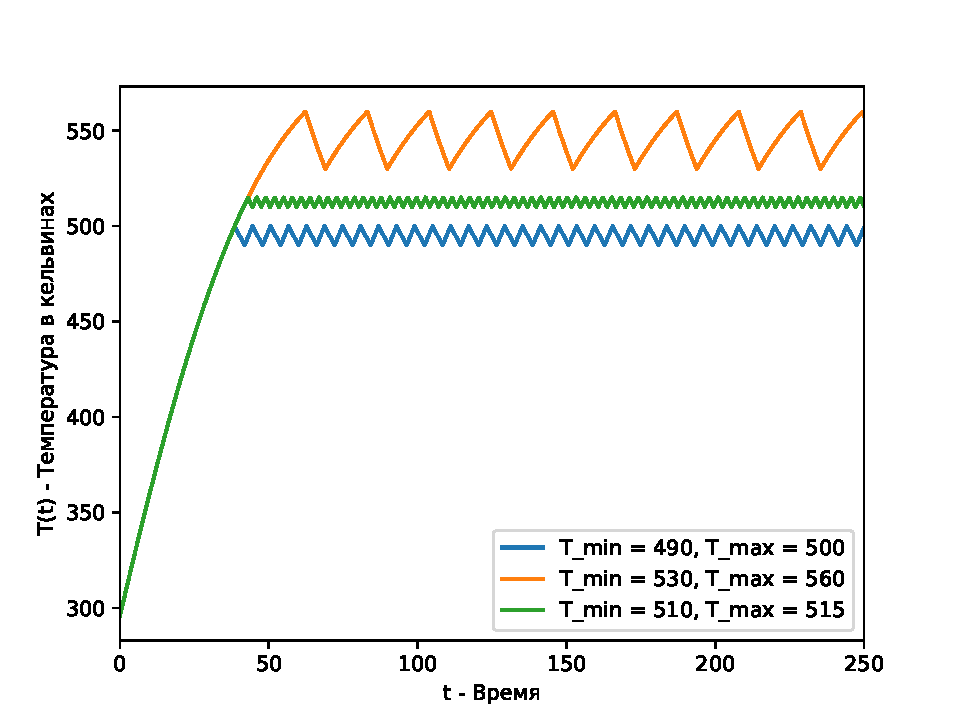
\includegraphics[width=12cm]{pictures/utug2.pdf}
            \caption{Графики моделей при $P = 3000 \text{Вт}, ~ m = 0.5 \text{кг}, ~ c = 897 \frac{\text{Дж}}{\text{кг} \cdot \text{К}}, ~ S = 0.4 \text{м}^2, ~ k = 2, ~ T_0 = 296 \text{K}$.}
        \end{figure}


        \begin{figure}[H]
            \centering
            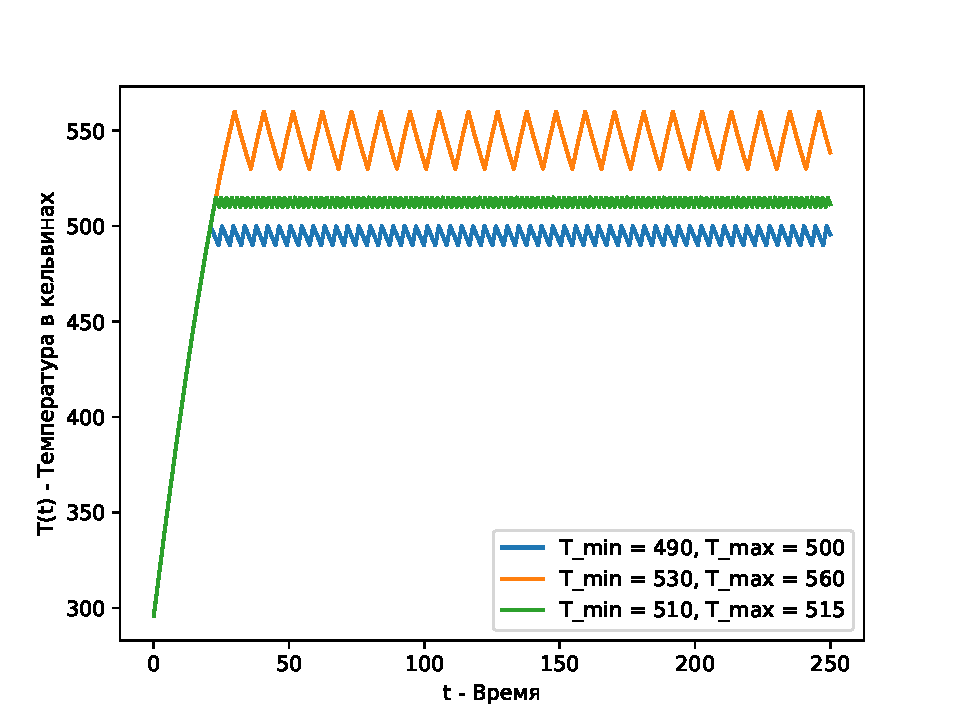
\includegraphics[width=12cm]{pictures/utug3.pdf}
            \caption{Графики моделей при $P = 2500 \text{Вт}, ~ m = 0.4 \text{кг}, ~ c = 554 \frac{\text{Дж}}{\text{кг} \cdot \text{К}}, ~ S = 0.2 \text{м}^2, ~ k = 4, ~ T_0 = 296 \text{K}$.}
        \end{figure}


        \begin{figure}[H]
            \centering
            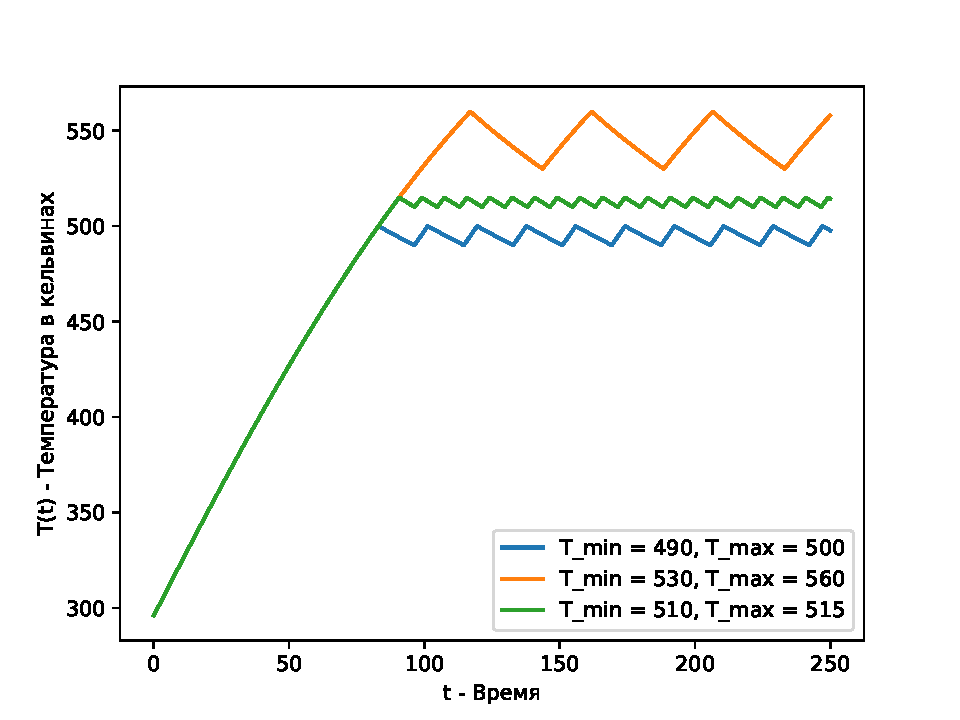
\includegraphics[width=12cm]{pictures/utug4.pdf}
            \caption{Графики моделей при $P = 2500 \text{Вт}, ~ m = 1 \text{кг}, ~ c = 897 \frac{\text{Дж}}{\text{кг} \cdot \text{К}}, ~ S = 0.2 \text{м}^2, ~ k = 2, ~ T_0 = 296 \text{K}$.}
        \end{figure}

        На (Рис. 2, 3, 4) построены модели, у которых отличаются только максимальное и минимальное значение температуры для функции-<<переключателя>>.

